%# -*- coding: utf-8-unix -*-
% !TEX program = xelatex
% !TEX root = ../thesis.tex
% !TEX encoding = UTF-8 Unicode

\chapter{系统测试}

对于任何软件,在完成了系统开发之后,都需要对系统进行测试,
以保证系统的质量。

\section{白盒测试}
本系统测试用例繁多,主要对以下几个较为重要的测试用例进行列举。
\begin{table}
	\centering
	\caption{添加任务测试用例表}
	\begin{tabular}{p{3cm}p{3cm}p{3cm}p{3cm}} \toprule
	  操作步骤 & 预期结果 & 实际结果 & 比较 \\
	  \midrule
	  点击新建任务 & 弹出新建任务界面 & 弹出新建任务界面 & 通过 \\ \midrule
	  在新建任务界面点击任意日期选择行 & 在选择行下方弹出日期选择器 & 在选择行下方弹出日期选择器 & 通过 \\ \midrule
	  在新建任务界面点击增加或减少精力等级 & 精力等级跟随变动 & 精力等级跟随变动 & 通过 \\ \midrule
	  在新建任务界面点击增加拆分项目 & 在拆分数量行下放添加拆分数量单位输入框,同时将估计花费时间改为估计单位花费时间 & 在拆分数量行下放添加拆分数量单位输入框,同时将估计花费时间改为估计单位花费时间 & 通过 \\ \midrule
	  在新建任务界面点击选择项目 & 弹出选择项目界面 & 弹出选择项目界面 & 通过 \\ \midrule
	  在选择项目界面点击选择项目 & 跳转回新建任务界面,同时更新项目和任务依赖选择 & 跳转回新建任务界面,同时更新项目和任务依赖选择 & 通过 \\ \midrule
	  在新建任务界面点击选择依赖任务 & 弹出选任务选择界面 & 弹出选任务选择界面 & 通过 \\ \midrule
	  在任务选择界面选择依赖任务并返回 & 保存依赖任务到内存中并更新依赖任务提示栏 & 保存依赖任务到内存中并更新依赖任务提示栏 & 通过 \\ \midrule
	  在新建任务界面点击完成 & 保存任务跳并转回原界面 & 保存任务跳并转回原界面 & 通过 \\ \midrule
	  在新建任务界面点击取消 & 不保存任务跳并转回原界面 & 不保存任务跳并转回原界面 & 通过 \\ \midrule
	  \bottomrule
	\end{tabular}
\end{table}

\begin{table}[!h]
	\centering
	\caption{用户完成含有拆分项目的任务用例表}
	\begin{tabular}{p{3cm}p{3cm}p{3cm}p{3cm}} \toprule
	  操作步骤 & 预期结果 & 实际结果 & 比较 \\
	  \midrule
	  点击完成任务 & 弹出新建行为界面 & 弹出新建行为界面 & 通过 \\ \midrule
	  在新建行为界面点击完成时间行 & 弹出日期和时间选择键盘 & 弹出日期和时间选择键盘 & 通过 \\ \midrule
	  在新建行为界面点击花费时间行 & 弹出倒计时时间选择键盘 & 弹出倒计时时间选择键盘 & 通过 \\ \midrule
	  在新建行为界面点击增加或减少精力等级 & 精力等级跟随变动 & 精力等级跟随变动 & 通过 \\ \midrule
	  在新建行为界面点击完成单位数量行 & 弹出数字键盘 & 弹出数字键盘 & 通过 \\ \midrule
	  在新建行为界面点击完成 & 保存行为跳并转回原界面 & 保存行为跳并转回原界面 & 通过 \\ \midrule
	  在新建行为界面点击取消 & 不保存行为跳并转回原界面 & 不保存行为跳并转回原界面 & 通过 \\ \midrule
	  \bottomrule
	\end{tabular}
\end{table}

\section{内存泄漏测试}
使用Xcode提供的Instruments对系统进行测试如图\ref{fig:memory_test}所示
\begin{figure}[!h]
	\centering
	\makebox[\textwidth]{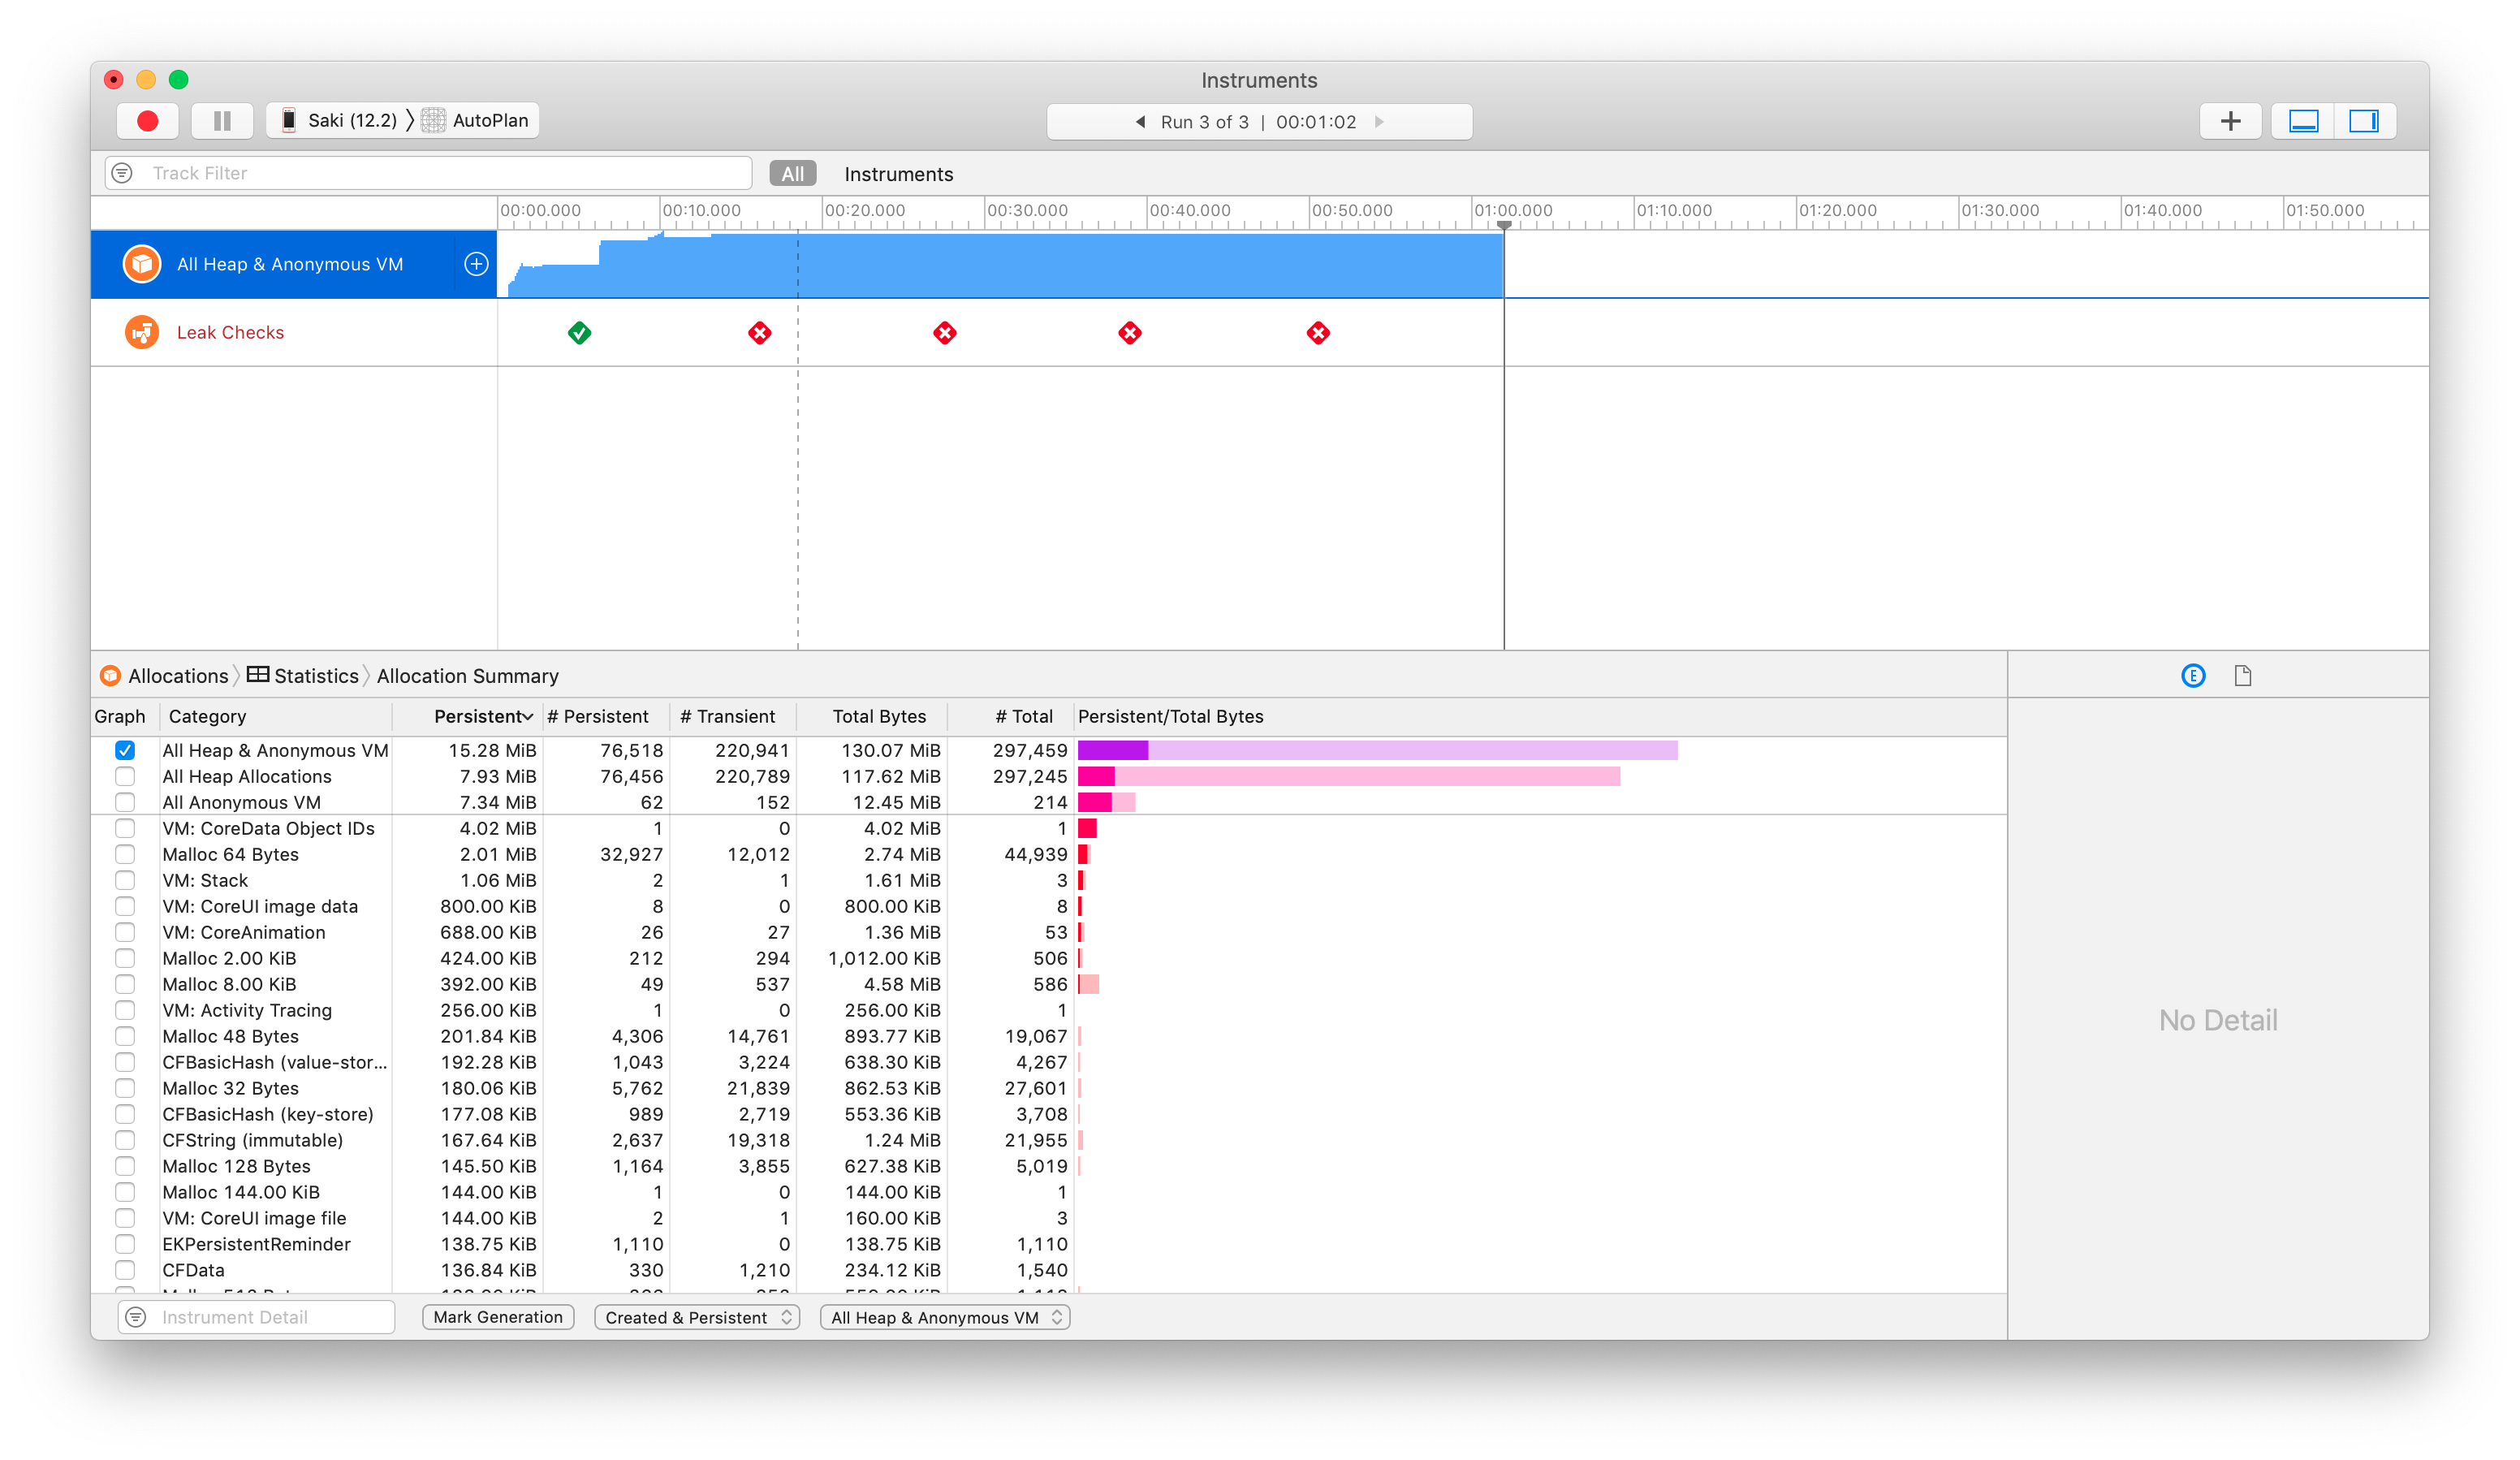
\includegraphics[width=\textwidth]{figure/test/memory_leak}}
	\caption{Instruments 内存泄漏测试}
	\label{fig:memory_test}
\end{figure}